%----------------------------------------------------------------------
% MAIN BODY
%----------------------------------------------------------------------

%======================================================================
\chapter{Inferential Roles and Distributed Representations}
%======================================================================
\renewcommand{\epigraphrule}{0pt}
\setlength{\epigraphwidth}{4.5in}
\epigraph{\textit{Neither Aristotelian nor Russellian rules give the exact logic of any expression of ordinary language; for ordinary language has no exact logic.}}{- P.F. Strawson, 1950}

\section{Introduction}

It is no secret that there are substantial dissimilarities between the formal languages of logic and the natural languages of everyday life \citep{Stanley:2008,Recanati:2012}. The former are precise and unambiguous, while the latter are rife with vagueness and context sensitivity \citep{Recanati:2012}. For philosophers interested in semantics, these differences give rise to a difficult methodological conundrum. On the one hand, it seems unlikely that a natural language can be assimilated to the structure of an underlying formal language, yet on the other hand, it seems unlikely that anything other than a formal language can provide us with the tools needed to describe the semantics of ordinary linguistic expressions. Formal languages are unfortunately the only languages for which we clearly know how to \textit{do}  semantics, and therefore provide the only available template for analyzing the meanings of words and sentences. So if Strawson is right to say that ordinary language cannot be understood in terms of the ``exact logic'' of a formal language, it is not clear how the construction of semantic theory ought to proceed. 

One option involves continuing the effort to find suitable correspondences between expressions in formal and natural languages. Truth-theoretic approaches to semantics proceed in roughly this fashion by identifying the underlying ``logical forms'' of linguistic expressions \citep{Soames:2010,Stanley:2008,Speaks:2014,Carpenter:1997}. Another option involves abandoning technical rigor in favor of analyses that seek to describe informal principles governing the use of ordinary language. But for those sympathetic to this broadly use-theoretic approach, the resulting lack of formal precision is a clear drawback. It becomes difficult to view semantics as a domain in which robust theories can be developed \citep[see][]{Wittgenstein:1953} 

The purpose of this chapter is to counter such pessimism by discussing a number of methods for mathematically characterizing the use-regularities that are evident in natural language. Drawn from the field of distributional semantics, these methods involve encoding statistical patterns gleaned from text into the elements of real-valued vectors to produce ``distributed representations'' of linguistic expressions \citep{TurneyPantel:2010,LandauerDumais:1997,Baroni:2014,Sahlgren:2005}. Such representations are widely used in the development of both natural language processing technologies and models of cognitive phenomena \citep{Manning:2015, LandauerDumais:1997,TurneyPantel:2010,Baroni:2014,JonesMewhort:2007,Fishbein:2008,Carrillo:2009}, but it's doubtful that they can independently satisfy the criteria outlined in the previous chapter. The problem is that a characterization of meaning involves giving a function specification in the form an inferential role, and distributed representations are not function specifications.\footnote{A ``distributed representation'' is for now best thought of as a vector that plays some role in some model that addresses some kind of loosely semantic phenomenon. In other words, it would be a mistake to assume that there is any well developed notion of semantics at work in the existing literature on distributed representations.} I nonetheless contend that the techniques of distributional semantics can be adapted to define models that learn to codify the meanings of certain linguistic expressions. More specifically, I argue that information about how sentences are distributed as premises and conclusions in a space of possible inferences can be used to build models that define inferential roles for arbitrary sentences. These inferential roles are in turn taken to determine the pragmatic significance of speech acts performed using particular sentences, as argued in Chapter 1.

In what follows, I first summarize the field of distributional semantics. Specifically, I examine connections between the goals of semantics discussed in the previous chapter and the so-called ``distributional hypothesis'' that provides the methodological underpinnings of this field. Next, I critically examine a number of distributional models that assign representations to words, phrases, and sentences on the basis of their statistical profile in a corpus of linguistic data. I then go on to discuss extended versions of these models that predict inferential relationships between sentence pairs, and thereby begin to formalize the notion of an inferential role. I conclude that the methods of distributional semantics, when appropriately extended to accommodate inferential contexts, allow for the development of use-theoretic approaches to meaning that are just as mathematically rigorous as their truth-conditional counterparts. 

\section{Distributional Semantics}

Distributional semantics is a loosely defined research area spanning linguistics, psychology, and computer science that is primarily characterized by the goal of describing the meanings of words\footnote{Phrases and sentences are something of an afterthought. See below for further discussion on this point.} in terms of their statistical distribution throughout the linguistic environment. The field's methodological roots are often traced back to Wittgenstein's (\citeyear{Wittgenstein:1953}) observations about the relationship between meaning and use \citep{Baroni:2014,TurneyPantel:2010}. To explain, the distributional approach takes to heart Wittgenstein's advice concerning the importance of cataloging how words are used by recording the frequency with which words occur in particular contexts. These frequency counts are then used to induce a similarity relation over words, on the assumption that words occurring in similar contexts tend to have similar meanings. This assumption is known as the ``distributional hypothesis'' in the literature \citep{Baroni:2014,TurneyPantel:2010,Sahlgren:2005}.

As described, the distributional hypothesis can seem to provide a rather unpromising starting point for the development of semantic theory. For one thing, the notion of a ``context of use'' is fairly vague and open to interpretation. For another thing, it is not immediately obvious that contextual co-occurrence provides good evidence of semantic similarity. The words ``doctor'' and ``stethoscope'', for instance, are likely to co-occur across a number of contexts, but their meanings are nonetheless quite distinct. Likewise, the words ``affluent'' and ``wealthy'' are roughly synonymous, yet they co-occur fairly infrequently because using both in the same context is often communicatively redundant. On the basis of these kinds of considerations, one might favor the weaker hypothesis that evidence of distributional similarity is at best evidence of some kind of minimal association between lexical items. 

The key to avoiding this weak characterization of the distributional hypothesis lies in getting clear on what counts as a context. One standard technique involves using collections of documents as contexts \citep[e.g.,][]{LandauerDumais:1997}. Then, counts of word occurrences in these documents are used to generate distributional profiles for lexical items. This strategy implements a variant of the distributional hypothesis on which words occurring in many of the same documents are assumed to have similar meanings. Another standard technique involves using nearby words as contexts (e.g., words in the same sentence as a target word). This strategy implements a variant of the distributional hypothesis on which words that co-occur in small windows of text are assumed to have similar meanings \citep[see e.g.,][]{JonesMewhort:2007,Sahlgren:2008,TurneyPantel:2010}. Additional context types used in the literature include word transition sequences \citep{JonesMewhort:2007}, syntactic neighborhoods \citep{Baroni:2014}, and relational contexts such as ``\textit{X} melts \textit{Y}'' that involve pairs of words \citep[see][p. 148-149]{TurneyPantel:2010}. 

Needless to say, the choice of context has a significant impact on the structure of the resulting word similarities. The use of documents as contexts, for instance, tends to produce word clusters that share a topical ``gist'' \citep{Baroni:2014}, while the use of words as contexts tends to produce word clusters with shared properties and taxonomical relatives \citep{TurneyPantel:2010}. The use of transition sequences as contexts tends to produce word clusters that correspond to grammatical classes \citep{JonesMewhort:2007}. While it is undoubtedly useful to be able to automatically induce such topical, taxonomical, and grammatical information from text corpora, it is not clear that the similarity relations that give rise to these clusters capture any genuine notion of meaning. It is for this reason that the notion of an \textit{inferential context} is used throughout this thesis to extend the techniques of distributional semantics in an appropriate manner.

It is also worth noting that there is a considerable amount evidence to suggest that ordinary distributional models can account for a wide range of psychological and linguistic phenomena. For instance, these models have been used to match human performance on tasks involving synonym identification \citep{LandauerDumais:1997} and analogical reasoning \citep{Plate:2003,Eliasmith:2001}. Distributional models have also been used to account for data from studies on linguistic priming, categorization behavior, and constraints on stem completion \citep{JonesMewhort:2007}. The breadth of these connections to empirical data suggests that the techniques of distributional semantics are more than just clever engineering tricks: they capture regularities in the statistical structure of the linguistic environment that people are undeniably sensitive to. So even though there is more to understanding a language than being sensitive to such regularities, distributional models are clearly capturing \textit{something} important about our linguistic knowledge.

To understand exactly what is being captured, it is important to examine the details of specific models from the literature. Upon doing so, it becomes clear that these models often learn to treat linguistic expressions as \textit{predictors} of other linguistic expressions. There is accordingly a natural connection between distributional semantics and the overarching theme in this work of thinking about linguistic expressions as informal instruments of prediction that, amongst other things, license inferences to other linguistic expressions.

\section{Word Embeddings}

Distributional methods for lexical analysis generate what are called ``word embeddings'' by mapping items from a preset vocabulary onto points in a continuous vector space. The mapping in question is typically designed so as to optimize some measure of accuracy in reconstructing or predicting raw word-context co-occurrence data recorded from the linguistic environment. To explain, this co-occurrence data is naturally represented in a space with as many dimensions as there are contexts under consideration (e.g., tens of thousands), while the word embeddings are represented in a space with considerably fewer dimensions (e.g., a few hundred).\footnote{The space containing the word representations is therefore ``embedded'' within the space containing the data.} The point of the embedding space is accordingly to provide a low-dimensional summary of this high-dimensional co-occurrence data. Designing the embedding space such that it can be used to reconstruct the raw data is simply a way of ensuring that the structure of the high-dimensional space is well preserved in its low-dimensional counterpart. 

Two general approaches to building low-dimensional embedding spaces are considered in what follows. The first, count-based approach operates by applying dimensionality reduction techniques to large collections of word counts, while the second, predictive approach operates by iteratively improving a procedure for predicting a word's context. In some ways, though, this is a distinction without a difference, since count-based and predictive models can be given roughly equivalent mathematical descriptions. 

\subsection{Count-Based Models}

Four steps are generally involved in producing a standard count-based word embedding model \citep{TurneyPantel:2010,LandauerDumais:1997,Baroni:2014}. First, one chooses a corpus of text from which to collect distributional information. Then, one chooses a context type (e.g., documents, words, etc.) and records word-context counts over the entire corpus. This procedure produces a co-occurrence matrix that has rows corresponding to words, columns corresponding to contexts, and entries that count the number of times a given word occurs in a given context. Third, the entries in this matrix are normalized or re-weighted to discount the presence of frequently occurring words (e.g. ``a'', ``the'') and to highlight the presence of rare but potentially informative words (e.g., ``carnivore'', ``saline'').\footnote{When documents are used as contexts, measures of pointwise mutual information or word frequency multiplied by inverse document frequency are typically used to normalize the word counts.} Finally, some form of dimensionality reduction is applied to the normalized co-occurrence matrix to extract low dimensional vectors corresponding to each word. This process usually involves computing the singular value decomposition of the matrix,\footnote{SVD factors a matrix into product of three matrices, the first of which is column orthonormal, the second of which is a diagonal matrix of singular values, and the third of which is row orthonormal. By eliminating all but the columns and rows of these matrices corresponding the highest \textit{k} singular values, a rank \textit{k} approximation of the original matrix is produced. This approximation is optimal in that it minimizes, given the approximation rank, the difference between the resulting matrix and the original matrix.} which makes it possible to compress word count information spread over numerous contexts into a relatively small number of dimensions.

One important benefit of performing dimensionality reduction is that similarities in the embedding space are induced on the basis of indirect or \textit{latent} co-occurrence relations in the original word count data \citep{TurneyPantel:2010,LandauerDumais:1997,JonesMewhort:2007}. Whenever two words occur in the same context, a constraint is introduced that favors locating their low-dimensional embeddings in close proximity to one another. But as more and more pairwise constraints of this sort are taken into consideration, the optimal distance between any two words in the embedding space will be determined in part by occurrences involving additional words. For instance, if word \textit{A} frequently occurs in the same contexts as word \textit{B}, and word \textit{B} frequently occurs in the same contexts as word \textit{C}, there will be pressure to locate the embeddings for \textit{A} and \textit{C} close to one another, even if \textit{A} has never occurred in the same context as \textit{C}. The reason this pressure arises is because the shortest distance between \textit{A} and \textit{C} cannot be greater than the sum of the shortest distances between \textit{A} and \textit{B}, and between \textit{B} and \textit{C}. So, to give a more concrete example, if the words ``doctor'' and ``veterinarian'' never occur in the same contexts, they might nonetheless have similar embeddings by virtue of both occurring in contexts containing a third word such as ``stethoscope'' \citep{LandauerDumais:1997,JonesMewhort:2007}. The overall point here is that the use of dimensionality reduction forces each word to be mapped into the embedding space in way to that best satisfies \textit{all} of the constraints imposed by the original co-occurrence data.

The fact that spatial relations between word embeddings are determined in this global manner has the interesting consequence of allowing a model to learn about a given word through exposure to data involving \textit{only} other words \citep{LandauerDumais:1997}. To illustrate with an example, imagine that our co-occurrence matrix is modified to include a number of new contexts in which the word ``stethoscope'' appears with names for other medical instruments such as ``scalpel'' and ``syringe''. The addition of this data forces the model to associate information about medical instruments with all of the words that have previously occurred in the same contexts as ``stethoscope'', for the reasons discussed in the previous paragraph. So, if ``doctor'' has previously co-occurred with ``stethoscope'', then the inclusion of the new information about medical instruments will act to subtly adjust the embedding for ``doctor'' to incorporate this information. This kind of indirect learning is very powerful. Landauer and Dumais (\citeyear[][pp. 223-26]{LandauerDumais:1997}) estimate that approximately three quarters of the structure present in an embedding space is due to latent rather than direct co-occurrence relations. Moreover, the existence of indirect learning provides concrete evidence that word embeddings generalize in a manner that is typically thought to be lacking in models that rely on association data.

There are, however, two major drawbacks to methods that produce word embeddings by performing dimensionality reduction on a co-occurrence matrix. First, there is no way to iteratively update the embedding space as more linguistic data becomes available, since the singular value decomposition of the entire co-occurrence matrix must be recomputed in order to incorporate any new information \citep{Sahlgren:2005}. Second, the resulting word embeddings contain no information regarding word order or syntax \citep{JonesMewhort:2007}. Each context is treated as a ``bag of words'', which entails that two contexts containing the same words in a different order are treated as identical. 

\begin{table}[!t]
\begin{center} 
\caption{Nearest Neighbors to Target Words using Count-Based Embeddings} 

\label{tab:nearestneighbors} 
\vskip 0.06in

\setlength{\tabcolsep}{13pt}
\begin{tabular}{llllllll} 
\hline

\multicolumn{2}{c}{\rule{0pt}{3ex} BRAIN} & 
\multicolumn{2}{c}{QUINE} & 
\multicolumn{2}{c}{FOOTBALL} & 
\multicolumn{2}{c}{HEART} \\
\hline
% \setlength{\tabcolsep}{1pt}
\rule{0pt}{3ex}brains & 0.74 & orman & 0.64 & league & 0.88 &
failure & 0.70  \\
tissue & 0.69 & quines & 0.60 & soccer & 0.81 &
suffering & 0.69  \\
lesions & 0.68 & analytic & 0.53 & leagues & 0.79 &
disease & 0.68  \\
causes & 0.67 & logical & 0.53 & fc & 0.79 &
death & 0.68  \\
abnormal & 0.66 & logic & 0.52 & club & 0.78 &
taken & 0.68  \\
\hline
\end{tabular} 
\end{center} 
\end{table}

More recently developed count-based methods avoid both of these problems. The key trick is to randomly assign an ``index vector'' in the embedding space to each item in a vocabulary, and then define the embedding for a given word as a linear combination of these index vectors \citep{JonesMewhort:2007,Sahlgren:2005,Sahlgren:2008}. This allows the embedding to be updated on the fly through changes to the underlying linear combination. Specifically, each time a target word is encountered in the corpus, its embedding vector (initialized as the zero vector) is updated with the sum of the index vectors for every other word in the surrounding sentence. Mathematically, the update corresponding to the $i^{th}$ occurrence of a target word is: 

\begin{equation}
v_{i}=v_{i-1}+ \sum_{j=1}^{n} {e_j}
\end{equation}

\noindent
where $v$ is the target word embedding, $e$ is an index vector, and $j$ is subscript ranging over $n$ words in the surrounding sentence. More intuitively, the embedding progressively shifts towards and away from particular index vectors as more and more text is analyzed, until eventually reaching a stable point. Examples of the resulting relations amongst embeddings are listed in Table \ref{tab:nearestneighbors}.\footnote{The examples in Tables \ref{tab:nearestneighbors} and \ref{tab:ordermodel} were generated from 25,000 Wikipedia articles using code available at https://github.com/pblouw/pysem.}

As Jones and Mewhort (\citeyear{JonesMewhort:2007}) illustrate, it is also possible to define index vectors that correspond to sequences of words (i.e., n-grams). The idea is to ``bind'' the index vectors for each word in a sequence into an index vector for the sequence itself. There are multiple ways to implement this sort of binding \citep[see e.g.,][]{Sahlgren:2008,JonesMewhort:2007,Blouw:2013}, but the simplest involves constructing index vectors for words occurring in particular positions relative to the target word. The linear combination defining a word's embedding is then updated on the fly to include sums of these positional index vectors. Mathematically, the sequence update for the $i^{th}$ occurrence of a target word is as follows:

\begin{equation}
v_{i}=v_{i-1}+ \sum_{j=1}^{n} {p_j \circledast e_{j} + p_{-j} \circledast e_{-j}}
\end{equation}

\noindent
where $v$ is again the embedding, $e$ is an index vector for a word, $p$ is an index vector for a position (e.g., two words to the right of the target word), and $j$ is subscript ranging over a window of $n$ words surrounding the target word. The $ \circledast $ symbol indicates circular convolution, which is an approximately invertable operation that is widely used to join vectors into simple structural arrangements \citep{Plate:2003}. Intuitively, it is again useful to think of the embedding progressively shifting towards and away from index vectors. In this case, however, each index vector corresponds to a word occurring in a particular neighboring position, and once the embedding reaches a stable point, it encodes a complex mixture of word sequences rather than word sets. The same technique can also be used to encode complex mixtures of syntactic structures instead of sequences. Table \ref{tab:ordermodel} illustrates some interesting ways in which the resulting embeddings can be manipulated.

\begin{table}[!t]
\begin{center} 
\caption{Phrase Completion using Count-Based Embeddings} 

\label{tab:ordermodel} 
\vskip 0.12in

\setlength{\tabcolsep}{13pt}
\begin{tabular}{lllllc} 
\hline

\multicolumn{2}{c}{\rule{0pt}{3ex} he \rule{0.25in}{.3pt} not} & 
\multicolumn{2}{c}{cognitive \rule{0.25in}{.3pt}} & 
\multicolumn{2}{c}{\rule{0pt}{3ex} Aristotle held more \rule{0.25in}{.3pt} theories}  \\
\hline
% \setlength{\tabcolsep}{1pt}
\rule{0pt}{3ex}did & 0.73 & meaningfulness & 0.48 & \quad \enspace sophisticated & 0.40 \\
does & 0.66 & dissonance & 0.47 & \quad \enspace manageable & 0.37 \\
do & 0.49 & neuroscience & 0.38 & \quad \enspace efficient & 0.37 \\
detests & 0.40 &  biases & 0.34 & \quad \enspace assertive & 0.37 \\
relished & 0.39 & neuroscientists & 0.29 & \quad \enspace stringent & 0.36 \\
\hline
\end{tabular} 
\end{center} 
\end{table}

\subsection{Predictive Models}

In recent years, researchers have largely abandoned count-based methods in favor of methods that directly learn to predict words from their surrounding contexts. The reasoning behind this shift is simple: word counts are collected because they can be used to predict the likelihood of word co-occurrences, but if so, then these word counts are mere proxies for the real measure of interest, which is co-occurrence likelihood. Predictive embedding models are thus designed to estimate this likelihood directly. 

Perhaps the most well-known example of such a model is the ``word2vec'' tool for creating word embeddings \citep{Mikolov:2013}. This tool is actually comprised of two parts: a continuous bag-of-words (CBOW) model that learns to predict a target word given a ``bag'' of surrounding words, and a skip-gram (SG) model that does just the opposite by learning to predict surrounding words from a single target word. Figure \ref{fig:w2v} illustrates the general architecture that is used by both models. In the case of CBOW, the input $x$ encodes a collection of context words, while the output $y$ is a probability distribution over the items in the model's vocabulary. The parameters of the model are iteratively adjusted so that output distribution $y$ maximizes the probability of the target word. In the case of SG, the input $x$ encodes a single target word, while the output $y$ is again a probability distribution over items in the model's vocabulary. This time, however, the parameters of the model are adjusted to maximize the joint probability of \textit{all} of the words in some collection associated with the target word. Both models operate on windows of text (e.g., spans of 7 words) drawn from a corpus.  

\begin{figure}
\centering
	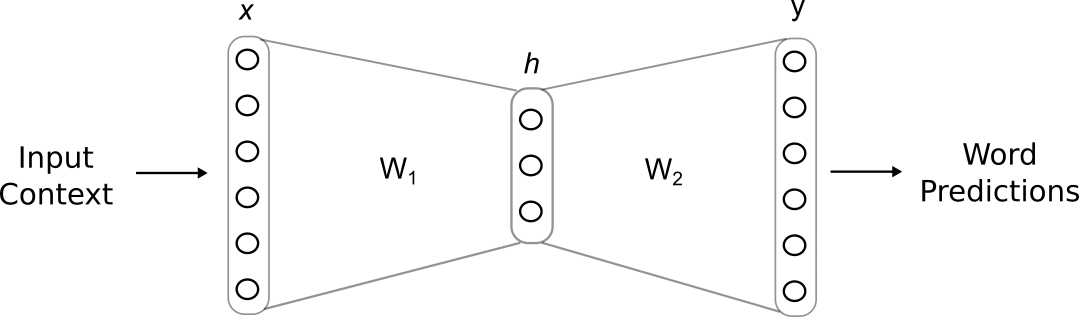
\includegraphics[width=4.5in]{figures/word2vec.png}
	\caption{Basic model architecture for learning word embeddings via prediction. A binary input vector, $x$, encodes a collection of one or more words that constitute a context. This input is then passed through a simple neural network that computes a probability distribution over words. Gradient descent is used to learn the weights $W_1$ and $W_2$ so that this probability distribution accurately reflects the likelihood of word co-occurrences in the training corpus. Embeddings for individual words correspond to the rows and columns of the weight matrices. Figure adapted from Rong (\citeyear{Rong:2014}).}
    \label{fig:w2v}
\end{figure}

In the special case where there is one target word and one context word, the CBOW and SG models are roughly equivalent. It helps to consider this case to obtain a deeper understanding of how these models work \citep[see][for further details]{Rong:2014}. Suppose a single word from a corpus is provided as the input context, $x$, and the next word in the corpus is the target for the output layer $y$.\footnote{It makes no difference to designate $x$ as the target and $y$ as the context, since both the target and the context are comprised of a single word here.} In this case, the input is encoded as a ``one-hot'' binary vector\footnote{A one-hot vector is a vector of zeros with a single element set to 1. This element corresponds to a particular feature of interest - in this case a single word.} that extracts a single column from the input-to-hidden weight matrix $W_1$. Thus, the value of the hidden layer is $h = W_1 x$, where $x$ is the binary input vector. Next, each unit in the output layer encodes a dot product between $h$ and a row in the hidden-to-output weight matrix $W_2$. The softmax function is then used to convert these dot products into a proper probability distribution. Importantly, each column of $W_1$ is treated as an embedding for a particular word, as is each row of $W_2$. The goal of learning is to make the $W_1$ embedding of a word most similar to the $W_2$ embedding of the target word that follows it in the corpus. 

At an intuitive level, the way that learning changes the model's weights is easy to understand \citep{Rong:2014}. Each row $j$ in $W_2$ is updated with values of the hidden layer activities, but scaled by both the learning rate and the prediction error at $y_j$. So, for a given output unit, if the model incorrectly guesses that the word corresponding to this unit ought to be predicted, the unit's incoming weights will be decremented to be more \textit{dissimilar} to the hidden layer vector. In effect, this lowers the value of the dot product between the first layer embedding of the input word, and the second layer embedding of the output word under consideration. On the other hand, if the model incorrectly fails to assign a high probability to the correct word, the unit corresponding to this word will have its incoming weights incremented to become more \textit{similar} to the hidden layer vector. This raises the value of the dot product between the first layer representation of the input word and the second layer representation of the correct output word. As such, when same input is provided again to the model, it will be more likely to predict the correct output. The updates to $W_1$ follow a similar but less directly interpretable pattern. Finally, the full CBOW and SG models both build on this basic procedure by either adding multiple words to the input or by attempting to predict multiple words at the output. 

\subsection{Discussion}

If talk of meaning is largely shorthand for talk of the expected effects of language use, then the idea of using continuous vectors to summarize linguistic regularities is an appealing one. An embedding can be thought of as a description of what is \textit{likely to follow} from the occurrence of a word, since measurements of embedding similarity are directly related to the conditional probability of one word appearing given another. As such, word embeddings are thematically consistent with the requirements of a semantic theory built on the idea that meanings specify certain expected consequences of language use. Understanding a language requires having a good predictive model of linguistic phenomena, and for all their simplicity, embedding models are nothing if not predictive.

It also possible to interpret embedding models as somewhat degenerate specifications of inferential roles. Prediction is a form of inference, so treating a word as a predictor of other words (as embedding models do) is equivalent to treating a word as something that licenses inferences to other words.\footnote{Strictly speaking, only sentences have inferential roles, since only sentences can be used as premises and conclusions in inferences \citep{Brandom:1994}. But prior to the discussion of compositionality in the next chapter, it is harmless to assume that words have inferential roles of the sort made explicit in conditional expressions such as ``If something is a robin, then it is a bird''.} The significance of this interpretation is that it suggests new responses to some standard criticisms of inferentialist approaches to semantics. For example, the fact that the inferential role of one expression cannot be defined independently of the inferential roles of numerous other expressions is often thought to problematically entail that no two language users share the same meanings, since no two language users will be disposed to make exactly the same inferences \citep{FodorLepore:1991,FodorLepore:2002}. Cast into the idiom of distributional semantics, the objection is that no two embedding models will possess exactly the same structure if they are generated from slightly different text corpora, and hence no two models will encode exactly the same meanings. But such models can nonetheless be highly \textit{similar} in the sense that they contain embeddings that are spatially distributed in a similar way. Moreover, it is possible to quantify this similarity such that if the models were taken to approximate human linguistic knowledge, it would be possible to make concrete estimates of the likelihood of successful communication. For instance, if two models assign the same ordinal ranking to the likelihoods of certain words co-occurring with a target word, then it's not clear that there are grounds on which to conclude that two speakers whose lexical knowledge is approximated by these models would ``misunderstand'' one another. Much more could be said here, but the point is simply to illustrate that a lot depends on the details of how one implements the notion of an inferential role. Dismissing inferentialist approaches on \textit{a priori} grounds is accordingly inappropriate.

It would nonetheless be a mistake to read too much into these models. For one thing, there is a world of difference between a word being used and a word merely occurring in particular context. Methods that aim to predict such occurrences accordingly do not explain language \textit{use} in the way that is required of theory of semantics. For another thing, these methods typically do not incorporate information that is relevant to explaining how linguistic expressions relate to the non-linguistic world. There is no in principle barrier to including such information \citep{Baroni:2014,LandauerDumais:1997}, but concrete efforts to do so are currently few and far between. Finally, the reason there has been a surge of recent interest in word embeddings has little to do with theoretical issues in semantics. Rather, embeddings have simply proven themselves to be useful ingredients in natural language processing tools such as parsers, part-of-speech taggers, and machine translation systems \citep{Manning:2015}. 

Overall, it is clear that embedding models can shed new light on longstanding issues in semantics concerning the viability of holism. But it is also clear that there remains a considerable gap between these models and a model that accurately captures the semantics of lexical items. Bridging this gap requires examining how words are combined to produce phrases and sentences.

\section{Phrase and Sentence Embeddings}

At first glance, it is not clear how to extend the distributional hypothesis to accommodate phrases and sentences. The problem is that multi-word linguistic expressions tend to be fairly unique and thus occur very rarely in the linguistic environment. Co-occurrence data then becomes highly \textit{sparse}, which makes it difficult to identify distributional regularities shared by multiple expressions \citep{Baroni:2014}. To illustrate this point with an example, it is likely that the previous sentence has \textit{never} occurred in written English before. The distributional profile of this sentence is accordingly difficult to compare to the profile of other sentences. 

However, it is possible to mitigate the effects of data sparsity by defining contexts that are shared by large numbers of distinct expressions \citep[][p. 261]{Baroni:2014}. One idea is to define these contexts in terms of words that are present in possible extensions of a target expression. For instance, the sentence ``the dog growled'' could be extended into ``the big dog growled and snapped its teeth'', which would then warrant treating the words ``big'', ``snapped'', and ``teeth'' as contexts defining the sentence's distributional profile. Another, similar idea is to use words occurring in sentences both before and after a target sentence as contexts. Interestingly, neither of these ideas has gained much popularity. Most researchers have instead chosen to develop methods for \textit{composing} the distributional profiles of words into distributional profiles for phrases and sentences \citep{Mitchell:2010,Baroni:2014}.

In what follows, I examine four approaches to composing word embeddings into phrase and sentence embeddings. The first approach uses additive operations to mix embedding components \citep{Mitchell:2010,Mikolov:2013}. The second approach uses multiplicative ``binding'' operations to join embeddings into simple role-filler structures \citep{SmolenskyLegendre:2006,Plate:2003,Eliasmith:2013,Smolensky:1990}. The third approach uses repeated applications of a single non-linear mapping to merge a set of embeddings in sequential order \citep{Elman:1990,Elman:1991}. Finally, the fourth approach generalizes the third to merge embeddings in accordance with a non-sequential structure such as a parse tree \citep{Socher:2014,Socher:2011,Tai:2015,Socher:2012,Iyyer:2014,Bottou:2014}. In addition to providing a deeper assessment of distributional approaches to semantics, this discussion helps to set the stage for a more thorough examination of compositionality in Chapter 4. 

\subsection{Additive Models}

In most early work on distributional semantics, vector addition is used as a sort of default method for producing composite embeddings. For instance, Landauer and Dumais (\citeyear{LandauerDumais:1997}) encode sentences as sums of word vectors in an effort to account for data from experiments involving assessments of paragraph coherence. Jones and Mewhort (\citeyear{JonesMewhort:2007}) similarly encode stems (i.e., multi-word prompts) as sums of word vectors in a effort to account for data from studies of constraints on stem completion. In more applied research on natural language processing, the use of vector addition to produce composite representations of sentences and documents is widespread.\footnote{Models that exploit addition to produce ``bag of words'' vector representations are often used as baselines to assess performance in tasks such as document classification. These baselines are often surprisingly hard to beat.} 

More recent work by Mitchell and Lapata (\citeyear{Mitchell:2010}) expands on this implicit use of vector addition by introducing a general class of additive composition functions. These functions all satisfy the following formula: 

\begin{equation}
v_{c} = \textrm{A}v_{s_1}+ \textrm{B}v_{s_2} 
\end{equation}

\noindent 
where $ v_{c} $ is an embedding for a complex expression, $ v_{s_1} $ and $ v_{s_2} $ are embeddings for simple expressions, and $ \textrm{A} $ and $ \textrm{B} $ are matrices (p. 1402). To provide some explanation, if $ \textrm{A} $ and $ \textrm{B} $ encode the identity transformation, then this approach is equivalent to vector addition. Otherwise, the contribution made by each constituent embedding is modulated to some degree. For instance, a head word\footnote{In linguistics, a head word is a word that provides a template of sorts into which obligatory arguments and optional modifiers are added to construct a complete phrase \citep{Pinker:1994,Harley:2014}.} might be given extra weight in the sum defining a phrase, so as to reflect its importance to the meaning of the phrase \citep{Baroni:2014}. Typical choices for $ \textrm{A} $ and $ \textrm{B} $ produce a weighted average or ``mixture'' of word embeddings \citep{Baroni:2014}.

Intuitively, these mixture models can be thought of as combining occurrence counts over contexts. For example, if the word \textit{A} occurs five times in some context while word \textit{B} occurs only two times, then the phrase \textit{AB} might be taken to occur in this context a total of seven times, or perhaps twelve times if \textit{A} is taken to be twice as important as \textit{B}. The advantage of combining contexts in this fashion is that the resulting embeddings retain information from each of their constituents. The drawback, of course, is that this information fails to capture how these constituents interact with one another. To say that an adjective-noun combination such as ``slow fish'' corresponds to an embedding that is comprised mostly of the embedding for ``fish'' does not provide much insight into the combination's distributional profile. A related problem is that function words such as ``on'' and ``the'' occur in almost every context, which means that they essentially just introduce noise into additive embeddings \citep{Baroni:2014}. Given the important semantic role played by function words, this consequence is undesirable. 

Overall, additive models tend to produce composite embeddings that cluster on the basis of weighted lexical overlap, and as such, the computed similarities tend only to capture coarse-grained topical relations. However, Mitchell and Lapata (\citeyear{Mitchell:2010}) report experimental results indicating that these relations correlate surprisingly well with human judgments of phrase similarity.  

\subsection{Multiplicative Models}

A slightly different approach to building composite embeddings emerges from early research on artificial neural networks. This work was frequently criticized for adopting representational assumptions inconsistent with the principle of compositionality \citep[see e.g.,][]{FodorPylyshyn:1988}, which prompted researchers to introduce methods for ``binding'' distributed representations together to form symbol structures \citep{Smolensky:1990,Plate:1995,Gayler:2004}. The most common method uses the tensor product\footnote{The tensor product of $ a \in R^m $ and $ b \in R^n $ is a tensor in $ R^{mn} $ whose elements are pairwise products of the elements in $a$ and $b$. It is equivalent to the outer product if $a$ and $b$ are vectors.} to produce ``role-filler pairs'' that tag particular representations to particular structural roles  \citep{SmolenskyLegendre:2006}.

Again, Mitchell and Lapata (\citeyear{Mitchell:2010}) expand on the notion of tensor product binding to introduce a general class of multiplicative composition functions. These functions all satisfy the following formula: 

\begin{equation}
v_{c} = \textrm{C} \cdot (v_{s_1} \otimes  v_{s_2})
\end{equation}

\noindent
where $ v_{c} $ is again an embedding for a complex expression, $ v_{s_1} $ and $ v_{s_2} $ are embeddings for simple expressions, $ \otimes $ is the tensor product, and $ \textrm{C} $ is tensor whose rank is greater than the rank of $ v_{s_1} \otimes  v_{s_2} $ (see pp. 1402-04 for details). If $ \textrm{C} $ is the identity, then the formula reduces back to the tensor product. If $ \textrm{C} $ is a binary tensor that extracts the diagonal of $ v_{s_1} \otimes  v_{s_2} $, then the formula is equivalent to the elementwise multiplication of $ v_{s_1} $ and $ v_{s_2} $. If $ \textrm{C} $ is a binary tensor with ones along the transdiagonal elements of its vertical ``slices'', then the formula computes the circular convolution of $ v_{s_1} $ and $ v_{s_2} $, which is equivalent to a compression of the tensor product \citep{Plate:2003,Mitchell:2010}. 

Intuitively, all of these variants can be thought of as generating occurrence counts for conjunctions of contexts. For instance, if word \textit{A} occurs in context \textit{X} two times while word \textit{B} occurs in context \textit{Y} three times, then the expression \textit{AB} is taken to occur six times in a conjunctive context \textit{XY}. In the special case where the composition function is element-wise multiplication, these conjunctive contexts are the same as the original contexts, which results in composite embeddings that accentuate points of overlap in the distributional profiles of their constituents \citep{Baroni:2014,Mitchell:2010}. Unsurprisingly, these multiplicative models have many of the same problems as their additive counterparts.

However, it is worth noting that multiplicative methods were not originally designed with the assumptions of distributional semantics in mind. Typical uses of tensor products and circulation convolution tend to define bindings between elements that are largely syntactic (i.e., roles) and elements that are largely semantic (i.e., fillers) \citep{SmolenskyLegendre:2006,Plate:2003}. Moreover, in the case of circulation convolution, binding is only guaranteed to work if the elements in each constituent vector take on values sampled from a mean-zero normal distribution \citep{Plate:2003}, which is unlikely to correspond to the occurrence statistics of any lexical item. The point here is that neither operation should be expected to combine distributional information in an intuitively plausible manner.

It is nonetheless worth pointing out that when multiplicative functions are combined with additive ones, it becomes possible to define complex symbolic structures using distributed representations. The specific choice of functions defines what is called a ``vector symbolic architecture'' or VSA \citep{Gayler:2004}. VSAs are used in cognitive models, but from a linguistic perspective, they are not entirely well-motivated \citep{Eliasmith:2013}. The problem is that a VSA defines complex linguistic expressions as collections of parts (i.e., specific role-filler bindings) that have no direct influence on one another. As will become clear, it is difficult to define inferential roles in terms of such role-filler collections. 

In all, the main drawback of both additive and multiplicative methods for producing complex embeddings is that they fail to adequately capture interactions between linguistic expressions \citep{Baroni:2014}. It is natural (and common in linguistics) to think of certain words as modifying other words. For instance, an adverb such as ``quickly'' modifies a verb it applies to by providing more specific information about the type of action the verb describes. Incorporating this kind of modification into composite embeddings requires the use of more complicated functions that operate over sequences and trees. 

\subsection{Sequential Models}

Sequential models for producing composite embeddings have their roots in research on recurrent neural networks (RNNs) in cognitive science and machine learning \citep{Elman:1990,Elman:1991}. These networks are mathematical models that map a series of inputs to a series of outputs by recursively applying a single non-linear function. Importantly, behavior of this function depends on both the current input to the network and the state of a ``hidden'' distributed representation that acts as a memory of prior inputs. The benefit of the feedback provided by this memory is that an RNN's hidden state becomes conditioned on the entire history of an input sequence. It is because of this sensitivity to input history that RNNs are used to model a wide range of sequential and temporally extended phenomena \citep{Sutskever:2014}. 

In linguistic applications, each input to an RNN corresponds to a word embedding, and the hidden state corresponds to composite embedding of all prior inputs. The recursion that defines this composite embedding is as follows:

\begin{align}
\label{eqn:rnn_hid}
h_t &= f (W^{xh} x_t + W^{hh} h_{t-1} + b) \\ 
\label{eqn:rnn_out}
y_t &= W^{hy} h_t 
\end{align}

\noindent
where $h_t$ corresponds to the current hidden state, $x_t$ corresponds to the input, $h_{t-1}$ corresponds to the previous hidden state, $b$ is a bias on the hidden state, and $f$ is an element-wise function. The matrices $W^{xh}$ and $W^{hh}$ apply transformations to the input and the previous hidden state, respectively. The output of the network, $y_t$, is then computed by applying the linear transformation $W^{hy}$ to the current hidden state.\footnote{Strictly speaking, computing a separate output from the hidden state is optional, so for simplicity I will assume that the composite embedding for a sequence of input embeddings is drawn from the hidden state.} The recurrence defined by these equations can be made more intuitive by unfolding it over a sequence to produce a chain of the sort depicted in Figure \ref{fig:rnn}. What is important to note is that equations (\ref{eqn:rnn_hid}) and (\ref{eqn:rnn_out}) define a composition function that produces embeddings with an internal structure defined by this chain, with the parameters $W^{xh}$ and $W^{hh}$ repeated at each link. Alternate composition functions that similarly unfold into a chain define alternate sequence models. A well-known example of such an alternative is the ``Long Short-Term Memory'' (LSTM) network \citep{Sutskever:2014}. 

\begin{figure}
\centering
	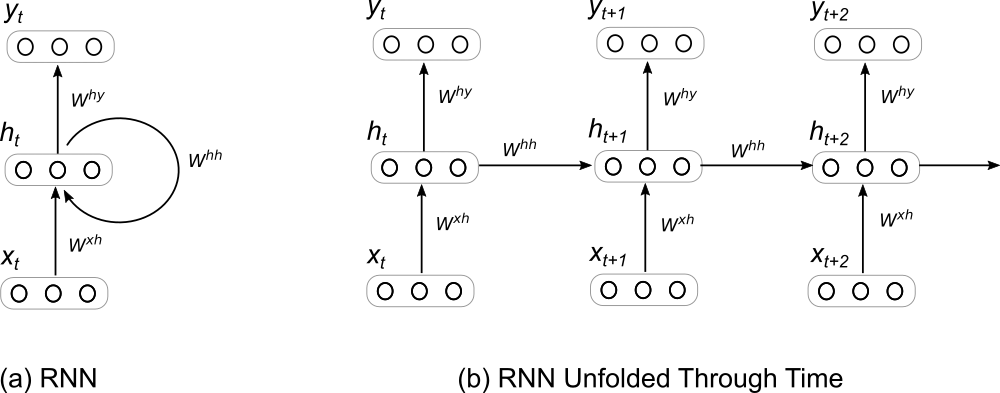
\includegraphics[width=5in]{figures/rnn.png}
	\caption{Unfolding a recurrent neural network through time. At each time step, an embedding corresponding to the current word in a sequence (e.g., a sentence) is provided as the input state $x$. The hidden state $h$ and the output state $y$ are then updated. Over time, $h$ and $y$ come to encode information about the entire history of the input sequence.}\label{fig:rnn}
\end{figure}

It is worth pointing out two things about the relationship between sequential, multiplicative, and additive models. First, if $f$ is set to the identity and $b$ is zero, then (\ref{eqn:rnn_hid}) is equivalent to an additive model that is applied over a sequence. If $W^{hh}$ is further set to compute a fixed circular convolution while $W^{hx}$ is set to the identity, then (\ref{eqn:rnn_hid}) can be thought of as implementing a VSA to produce a simple list. These observations indicate that sequential models implement some (though not all) simpler composition functions as special cases. Second, the recursive nature of these models allows them to accommodate the idea that linguistic expressions modify one another. More specifically, it is possible to think of a recurrent network as a function whose behavior is defined by its previous inputs. Thus, when a new input is presented, it is in a sense \textit{modified} by all previous inputs to yield the next state of the network. It is for this reason that RNNs have to the power to capture complex sequential dependencies between words \citep{Elman:1991,Sutskever:2014}.

Unlike most additive and multiplicative models, RNNs do not compute functions that are defined \textit{a priori}. They are instead trained to \textit{approximate} an unknown function by learning from examples of the function's inputs and outputs. Details of the training procedure can vary, but typically the backpropogation method is used in tandem with gradient descent to find a set of parameters that minimize some measure of error in the network's outputs. There are, however, two drawbacks to this kind of training when it is applied to the problem of producing embeddings for word sequences. First, examples of good multi-word embeddings are needed to provide the necessary training data. It is often not clear what such examples should look like, and even when it is, they are typically hard to come by in sufficient quantity. Second, it is difficult to interpret the hidden states of an RNN once its parameters have been optimized. The dimensions of this state typically have no direct interpretation as occurrence counts in particular contexts, which makes it unclear how to understand RNN embeddings in distributional terms. 

A more theoretical problem is that there are good reasons to think that linguistic structure is non-sequential. The possibility of arbitrarily iterated noun phrases such as ``the big dog with the leather collar with the shiny tag with the...'' that eventually combine with a verb phrase has motivated numerous views on which linguistic expressions are organized into hierarchies rather than sequences \citep{Pinker:1994,Harley:2014}. While RNNs fail to capture this hierarchical structure, they can be generalized to create fully recursive models that unfold into trees and certain other kinds of graphs \citep{Socher:2012,Socher:2014,Bottou:2014}. 

\subsection{Tree-Structured Models}

Tree-structured models differ from sequential models by defining composition functions that map variable numbers of ``child'' embeddings onto a single ``parent'' embedding. For example, the embeddings for the child words ``no'' and ``thesis'' might be mapped by a single function to produce an embedding for the parent noun phrase ``no thesis''. Further applications of this function can then be used to produce an embedding for the verb phrase ``writes itself'' from embeddings for each of its constituents, along with an embedding for the sentence ``no thesis writes itself'' from embeddings of the resulting noun and verb phrases. The advantage of these kinds of functions is that they allow word embeddings to be composed in accordance with the syntactic structure of a sentence and therefore accommodate standard linguistic analyses of the interface between syntax and semantics \citep[see e.g.,][]{Szabo:2012}. 

It is also possible to define composition functions that accommodate a variety of different of syntactic formalisms. For instance, functions defined over pairs of child embeddings are consistent with binary constituency grammars \citep{Socher:2012}, while composition functions defined over variable numbers of child embeddings are consistent with dependency grammars \citep{Socher:2014,Tai:2015}. Furthermore, the use of typed lexical embeddings (i.e., embeddings that reside in different vector spaces) can be used to define composition functions consistent with categorial grammars, wherein certain linguistic expressions are treated as functions that get applied to other linguistic expressions \citep{Baroni:2014}. A standard RNN, finally, is a special case of a tree-structured model in which the tree is binary and strictly left-branching. Figure \ref{fig:tree-rnn} illustrates examples of different tree structures and their corresponding composition functions. 

\begin{figure}
\centering
	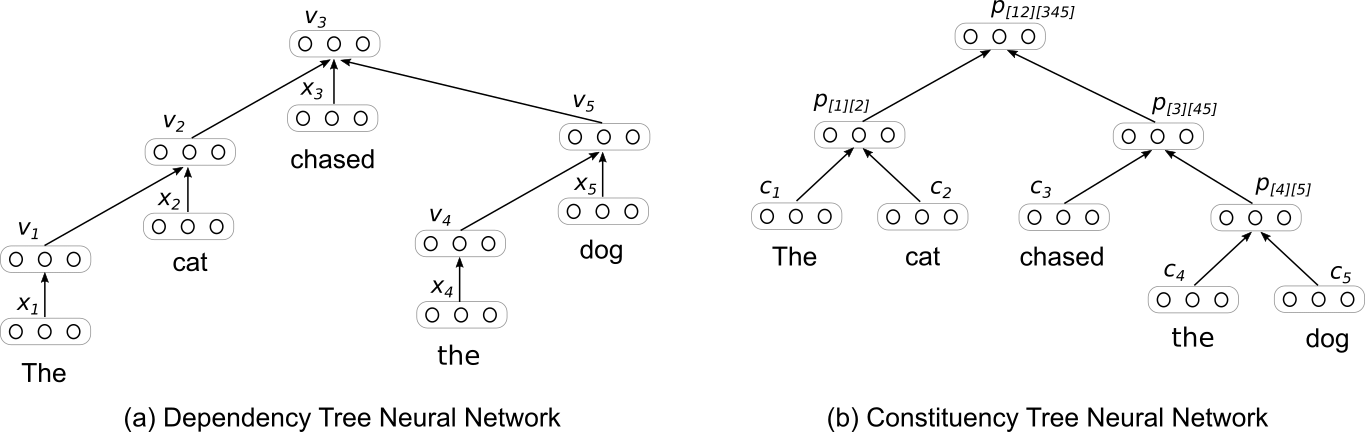
\includegraphics[width=6in]{figures/tree_comp.png}
	\caption{A comparison of dependency and constituency tree structured neural network models. In each case, a network layout is constructed from a parse of the input sentence. Constituency-based networks include layers corresponding to phrasal constituents (e.g., noun phrases), while dependency-based networks do not. Variables are labeled for consistency with the naming conventions in equations (\ref{eqn:ct_rnn}), (\ref{eqn:dt_rnn_leaf}), and (\ref{eqn:dt_rnn_nonleaf}), which formally describe how sentence embeddings are produced using each model.}
\label{fig:tree-rnn}
\end{figure}

Given that these models apply a composition function in a hierarchical manner to produce a single embedding for a sequence of words, it follows that some prior specification of the structure of this hierarchy must be provided. It is for this reason that many tree-structured models rely on external parsers to define a layout for the neural network that is used to produce a sentence embedding from a set of word embeddings \citep{Socher:2012,Socher:2014}. Once this layout is produced, it is relatively straightforward to compute embeddings for both the sentence as a whole and its various constituents. In the case of a binary constituency tree, the standard composition function used to produce these embeddings is the following:

\begin{align} 
\label{eqn:ct_rnn}
v_p = f (W [v_{lc}; v_{rc}] + b)
\end{align}

\noindent
where $v_p$ is the parent embedding, $[v_{lc}; v_{rc}]$ is the concatenation of the left child embedding and the right child embedding, $b$ is a bias on the parent embedding, $f$ is an element-wise function, and $W$ is a matrix that maps the concatenated embedding back into the space of the child embeddings. This composition function is then applied recursively to compute embeddings for each node in the tree whose children have been computed, and the recursion terminates when every node in the tree is assigned an embedding. As in the case of sequential models, an external error signal of some kind is typically used to learn the parameters of the composition function, in this case the matrix $W$ and the bias vector $b$. More complicated composition functions with larger numbers of parameters are also possible \citep[e.g.,][]{Tai:2015,Socher:2012}, provided that they map two child embeddings to a single parent embedding of the same dimensionality. 

One drawback of constituency trees is that they produce embeddings that are quite sensitive to subtle changes in word order and word choice, even if the resulting sentences are highly similar \citep{Socher:2014,Iyyer:2014}. For example, the constituency trees for passive and active variants of the same sentence are quite distict (e.g., ``Paul played the piano'' vs ``The piano was played by Paul''), which can lead a model to produce fairly dissimilar embeddings using these trees \citep{Socher:2014}. Another drawback is that embeddings at the nodes closest to the root of a constituency tree tend dominate the overall sentence embedding. This is undesirable if the nodes in question correspond to words or phrases that are minimally important to the sentence's meaning \citep{Socher:2014}.

Models that make use of dependency trees rather than consituency trees avoid most of these problems \citep{Socher:2014}. A dependency tree assigns a single node to each word in a sentence, and then introduces a set of edges (or ``arcs'') that identify which nodes depend on other nodes to be interpreted properly. A \textit{root} node that depends on every other node in the tree (either directly or indirectly) is then taken to summarize the entire sentence. A constituency tree, in contrast, has one \textit{leaf} node per word in a sentence, plus numerous intermediary nodes that correspond to phrases or phrasal constituents that eventually combine produce a root node for the sentence as a whole. So, in the case of sentence with \textit{n} words, a dependency tree will consist of \textit{n} nodes, while a binary constituency tree will consist of $2n - 1$ nodes. Dependency trees are accordingly relatively shallow in comparison to constituency trees. This can be advantageous when use training algorithms that rely on backpropogation. Example dependency and constituency trees are shown in Figure \ref{fig:tree-rnn}. 

A further advantage of using dependency trees is that the links between nodes are labeled with specific dependency relations that can be used to parameterize a composition function. Specifically, each dependency relation is associated with a specific weight matrix that is used to help determine the embedding. The assignment of embeddings to nodes in the tree then proceeds in a two-step manner. First, all of the leaf nodes in the tree (i.e., nodes that do not depend on other nodes) are assigned embeddings by applying a simple transformation to their underlying word embeddings:

\begin{align} 
\label{eqn:dt_rnn_leaf}
v_j = f (W_v x_j + b) 
\end{align}

\noindent
where $v_j$ is the embedding for the $j^{th}$ leaf node in the tree, $x_j$ is the embedding for the word corresponding to this node, $W_v$ is a matrix that transforms word embeddings, and $b$ and $f$ are a bias term and elementwise function as before. Second, embeddings are recursively assigned to all of the non-leaf nodes by composing the embeddings of their children as follows:

\begin{align}
\label{eqn:dt_rnn_nonleaf}
v_i = f (W_v x_i + b + \sum_{j \in C(i)} W_{R(i,j)} \cdot v_j )
\end{align}

\noindent
where $v_i$ is the embedding for the $i^{th}$ non-leaf node in the tree, $x_i$ is the embedding for the word corresponding to this node, $j$ is an index that ranges over the children, $C(i)$, of node $i$, and $W_{R(i, j)}$ is a matrix associated with the specific dependency relation between node $i$ and its $j^{th}$ child. $v_j$ is the embedding corresponding to this child. One thing to note about this formalization is that the composition function is invariant to changes in the order of the words corresponding to its children. For instance, encodings of the phrases ``a gray bellowing hippo'' and ``a bellowing gray hippo'' will assign identical embeddings to the head word ``hippo''. Whether or not this kind of order invariance constitutes a problem probably depends on the task to which the model is applied.

As before, the use of error-driven parameter learning requires that a model be provided with examples of desirable sentence embeddings. Most tree-structured neural networks are accordingly parameterized for a very specific task, such as predicting sentiment labels for sentences \citep{Socher:2011,Socher:2012}. This kind of task-specificity is not necessarily a problem, but it does raise the question of whether it is possible to create generic embeddings that are able to account for a wide range of semantic phenomena.

\subsection{Discussion}

Care is required in giving semantic interpretations of phrase and sentence embeddings. These embeddings typically reside in the same vector space as the word embeddings from which they are derived, so it is theoretically possible to interpret them in distributional terms. Each element of a word embedding, recall, corresponds to a measure of its likelihood to occur in an abstract context.\footnote{The contexts are abstract in the sense that they are defined through the application of a dimensionality reduction procedure to a co-occurrence matrix.} Different composition functions (i.e., additive, tree-structured, etc.) define different ways of assigning values to the elements in one vector on the basis of the values of elements in a set of \textit{other} vectors. So, there is a natural sense in which these functions determine the distributional profile for a complex expression from the distributional profiles of its simpler parts. The methods under consideration accordingly compose distributional profiles in a manner analogous to to the way in which truth-theoretic approaches compose denotations by computing the denotation of a complex expression from the denotations of its simpler parts \citep{Carpenter:1997}. 

There are two problems with this straightfowardly compositional view of sentence embeddings. First, when an error signal is used to define a composition function, the embeddings produced by this function take on values that minimize the magnitude of the error signal. So, if the error signal is not designed to produce good distributional profiles for multi-word expressions, then it is simply a mistake to interpret the resulting embeddings in distributional terms. Second, even if the error signal is described in terms of antecedently specified distributional profiles, one is still stuck with the problem of choosing appropriate contexts over which to define these profiles, as discussed in the introduction to this section. The use of nearby words as contexts does allow one to specify distributional profiles for simple multi-word expressions \citep[see][pp. 290-295]{Baroni:2014}, but this choice is poorly motivated from a theoretical perspective. Co-occurrence events involving single words essentially become primitives for semantic analysis at every level of syntactic complexity, and such primitives are surely inadequate if the goal of semantics is to explain how words and sentences function as complex tools for prediction in social contexts that involve intentional interpretation. 

The best way to think about these methods is in terms of the fact that different composition functions induce different similarity relations over the linguistic expressions for which embeddings are produced. Additive models typically define this similarity relation in terms of a weighted lexical overlap between two expressions, while multiplicative models define it in terms of prominent conjunctions of embedding elements. Both kinds of model are usually unsupervised in the sense that they are not trained to produce embeddings that satisfy some external criterion. Sequential and tree-structured models, in contrast, are neural networks that do rely on such a criterion. In standard cases, the relevant criterion is to minimize some measure of error in predicting the correct network outputs for some set of example network inputs. The inputs in this case would be sentences and the outputs might be classification judgments of some kind. By minimizing its prediction error, a model learns to approximate some undefined function from sentences to class labels, where the training input-output pairs are taken to be sampled from this function. The key point here is that the similarity relation induced over a set of linguistic expressions is determined by the specific function being approximated.

One interesting feature of these induced similarity relations is that they are all consistent with the previously mentioned idea of treating linguistic expressions as predictors of other linguistic expressions (or their properties). To explain, if a similarity relation is induced on the basis of distributional information, then measurements of embedding similarity are again related to the conditional probability of one expression appearing given another. Alternatively, if a similarity relation is induced through function approximation, then measurements of embedding similarity are related to the conditional probability that one expression gets mapped to a particular output given that another does. The difference between these two cases is that in one, expression occurrences are being predicted, while in the other, function outputs are being predicted. 

So, in keeping with the idea that describing an expression's meaning involves giving a specification of the expected effects of its use, the correct way to interpret these sentential embeddings is in terms of the role they play in regulating the functional behavior of the models in which they are defined. For instance, in an unsupervised additive model, sentence embeddings regulate predictions of sentence similarity. Similarly, in an supervised sequence model, sentence embeddings regulate predictions of sentence labels. Unfortunately, none of the models discussed here rise to the challenge of defining functional behavior that captures the pragmatic significance of uttering a linguistic expression. Again, this pragmatic significance is to be understood in terms of a sentence's inferential role, so the clear next step involves building models that predict inferential relationships between sentences.  

\section{Predicting Inferential Relationships}

As Brandom (\citeyear{Brandom:1994}) notes, semantics must answer to pragmatics (p. 83). The pragmatic significance of uttering a particular sentence is characterized by the IPA framework in terms of the effect the utterance has upon a conversation. This effect, again, determines which further claims each interlocutor can be expected to assent to, which questions they can be expected to ask, which commands they can be expected to issue, and so forth. An inferential role is then introduced to codify such effects, and thereby explain how the sentence is \textit{used} to anticipate and control the trajectory of a dialogue. Talk of meaning is accordingly talk of how linguistic expressions function as instruments of prediction in the context of intentional interpretation.  

If the distributional methods just discussed are to account for how linguistic expressions function as such instruments, then they obviously need to be extended considerably. I suggest a two step approach to performing this extension. The first step involves formulating the notion of an inferential role in terms of a function that maps a sentence onto the further sentences that follow from or contradict it. These sentences constitute a kind of ``local neighborhood'' around a target sentence within a much broader network of inferences. The second step involves approximating the function that produces this local neighborhood by using an embedding model that learns from training examples. If successful, this two step process will yield a model that is able to compute rudimentary inferential roles for arbitrary input sentences. 

The viability of this approach hinges on the use of high quality training data. In what follows, I first discuss a recently released corpus that provides such data. I then describe sentence embedding models that learn on the basis of this data to predict inferential relationships between sentences. Next, I present results that illustrate how well each model is able to predict relationships between novel sentences not seen in the training data. I conclude by illustrating how these models can be used to construct a simple inferential network around a target sentence.  

\subsection{The SNLI Corpus}

The Stanford Natural Language Inference (SNLI) corpus is a recently released dataset consisting of 570,152 sentences pairs labeled with inferential relationships \citep{Bowman:2015}. The first sentence in each pair is referred to as the \textit{premise}, while the second sentence is referred to as the \textit{hypothesis}. If the hypothesis follows from the premise, then the pair is labeled as an example of entailment. If the hypothesis is inconsistent with the premise, the pair is labeled as an example of contradiction. And if the hypothesis might or might not be true given the premise, then the pair is labeled as neutral.

Each sentence pair is generated by providing a human annotator\footnote{These annotators were recruited through Amazon Mechanical Turk. See Bowman et al. (\citeyear{Bowman:2015}) for details.} with an image caption (but not the corresponding image), and then asking them to write three further captions: one which is definitely also true of the image, one which might be true of the image, and one which is definitely not true of the image. To illustrate with an example, one initial caption is ``Under a blue sky with white clouds, a child reaches up to touch the propeller of a plane standing parked on a field of grass,'' and the annotator produced the following three additional captions: ``A child is reaching to touch the propeller of a plane'' (entailment), ``A child is reaching to touch the propeller out of curiosity'' (neutral), and ``A child is playing with a ball'' (contradiction). The use of image captions is designed to eliminate ambiguities concerning event and entity co-reference across the sentences in a given pair. Approximately ten percent of resulting pairs were subject to further validation step in which four additional annotators assigned them one of the three relationship labels. The results of this data validation suggest that inter-annotator agreement is very high, with approximately 98\% of validated sentence pairs receiving a consensus label (i.e., at least three of the five annotators are in agreement). 

Finally, the dataset is divided into a training set of 550,152 sentences pairs, a development set of 10,000 pairs, and a test set of 10,000 pairs. The training set is used to teach a model to assign the correct inferential labels to sentence pairs, while the test set is used to assess how the well the resulting model is able to assign labels to novel pairs. The development set is used to select model hyper-parameters (i.e., parameters that are not learned over the course of training, such as the embedding dimensionality). 

\subsection{Model Details}

To compare different sentence embedding models, I ran a series of experiments assessing performance on the SNLI task. Specifically, I test four models: (1) an additive model that encodes each sentence as a sum of word embeddings; (2) a multiplicative model that encodes each sentence as a collection of role-filler pairs; (3) a sequential model that encodes each sentence using an RNN; and (4) a tree-structured model that encodes each sentence using a network constructed with the help of a dependency parser. For each sentence pair, these models are used to create two sentence embeddings, which are then concatenated into a single embedding that is passed to a simple feed-forward neural network that acts as a classifier by computing a probability distribution over possible labels. Figure \ref{fig:model} illustrates this model architecture in more detail.

The models are all trained via backpropogation to learn a set of parameters for both the classifier and the sentence embedder that minimizes error on the training set. All of the models are initialized with 300 dimensional word embeddings created using the methods of Mikolov et al. (\citeyear{Mikolov:2013}). These word embeddings are then fine-tuned over the course of training. Each model was trained for approximately twenty passes over the entire training set, with the learning rate annealed by half after every three passes. The same embedding model is used for both the premise sentence and the hypothesis sentence in all cases. A description of further details concerning these experiments, along with the code used to run them, is available online at https://github.com/pblouw/pysem. 

\begin{figure}
\centering
	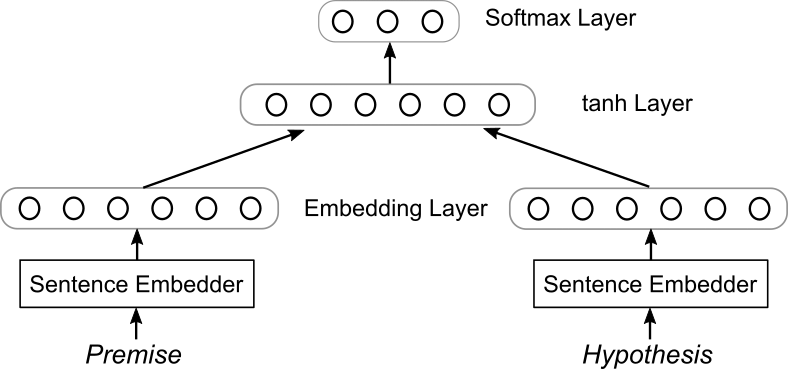
\includegraphics[width=3.8in]{figures/classifier.png}
	\caption{General model architecture for predicting inferential relationships between pairs of sentences \citep[see][]{Bowman:2015}. The premise and hypothesis sentences are each embedded using one of the models described in Section 2.4 above. The resulting embeddings are concatenated and fed into a simple neural network that performs a three-way classification (entailment, contradiction, or neutral) using a single tanh hidden layer and a softmax output layer.}\label{fig:model}
\end{figure}

\subsection{Results and Error Analysis}

The accuracy of each model on the training set and the testing set is presented in Table \ref{accuracy}. As is clear, the multiplicative model performs the worst, with the remaining models performing fairly comparably on the test data. The tree-structured model, however, is unique in that it performs very well on the training data. This high performance is almost certainly a case of overfitting, since the model has a vast number of free parameters, and since performance on the test data is comparatively low. However, it should be possible to reduce this overfitting by either (a) introducing regularization, (b) reducing the number of model parameters, or (c) increasing the amount of training data. I accordingly focus primarily on the use of this tree-structured model in what follows, since it is both linguistically well-motivated and empirically successful.

There are at least three kinds of sentence pairs that this tree-structured model tends to have difficulty with. First, if one of the sentences is extremely long, the model seems to be unable to identify information that is relevant to determining its relationship to the other sentence. For example, in the test case where the premise sentence is ``a group of young boys wearing track jackets stretch their legs on a gym floor as they sit in a circle'', while the hypothesis sentence is ``the boys in their track jackets in the gym stretch their legs'', the model incorrectly predicts a contradiction, presumably because it cannot determine whether talk of sitting or stretching in the premise sentence ought to be used to evaluate the likelihood of the hypothesis sentence. Second, if the inferential relationship between two sentences is determined by sophisticated forms of background knowledge that the model is not able to induce from the training data, then model is likely to make an incorrect prediction. For example, in the test case where the premise is ``a man in a short mohawk and beard'', while the hypothesis is ``there is a man with a ponytail and a mustache'', the model incorrectly predicts an entailment, since it has no way of knowing that a mohawk is a hairstyle that is distinct from a ponytail. Third, if an inferential relationship between two sentences is determined by complex scoping relations involving negations or quantifiers, then the model is again likely to make an incorrect prediction. In the test case where the premise is ``a group of men are sitting and standing a courtyard, some of them are reading books and some are talking'', while the hypothesis is ``a group of males are outside reading and singing'', the model incorrectly predicts an entailment, presumably because it fails to grasp that the double use of the word ``some'' splits the group into those who talk and those who read, thereby ruling out the existence of a group that both sings and reads. Improving the model's ability to handle these kinds of cases likely requires the use of a more varied selection of training data.  

\begin{table}[!t]
\begin{center} 
\caption{Model Accuracies on the SNLI Classification Task} 
\label{accuracy} 
\vskip 0.12in
\begin{tabular}{c c c c} 
\hline
Model & Parameters &  Training Set (\%)  & Test Set (\%)\\
\hline
Chance  & 0 & 33.3 &  33.7 \\
Additive & 181,200 & 79.2 & 76.7 \\ 
Multiplicative & 181,200 & 58.6 & 59.2 \\
Recurrent & 361,800 &  75.6 & 75.0  \\
Tree-Structured &  4,334,700 &  83.7 & 77.0  \\
\hline
\end{tabular} 
\end{center} 
\end{table}

One interesting feature of the model is that it can be used to iteratively construct a sentence's inferential role. The construction procedure involves applying the model to a series of sentence pairs in which some sentence of interest is held constant as either the premise or the hypothesis. The predictions of the model can then be used to build out networks of the sort depicted in Figure \ref{fig:infrole}. These predictions are not universally correct, as is shown by the fact the model incorrectly predicts an entailment relation in cases where the hypothesis sentence is very likely, but not guaranteed, to follow from the premise sentence. For example, the model predicts that the sentence ``The kids are outside'' is entailed by the sentence ``some kids are wrestling on an inflatable raft'', which discounts the possibility that the kids are in an indoor pool.

The most important thing to note about these results is that, for each premise sentence, the model places \textit{every} other possible sentence into one of three disjoint classes: one corresponding to sentences that follow from the premise, one corresponding to sentences that contradict the premise, and one corresponding to sentences that are neutral with respect to the premise. Given as much, it is reasonable to conclude that the model can be used to assign a rudimentary inferential role to every possible sentence that can be formed using a vocabulary of known words. These inferential roles may not perfectly codify the correct uses of particular sentences, but they do provide a good foundation for building towards technically rigorous approaches to semantics that follow in the use-theoretic tradition.  

\begin{figure}
\centering
	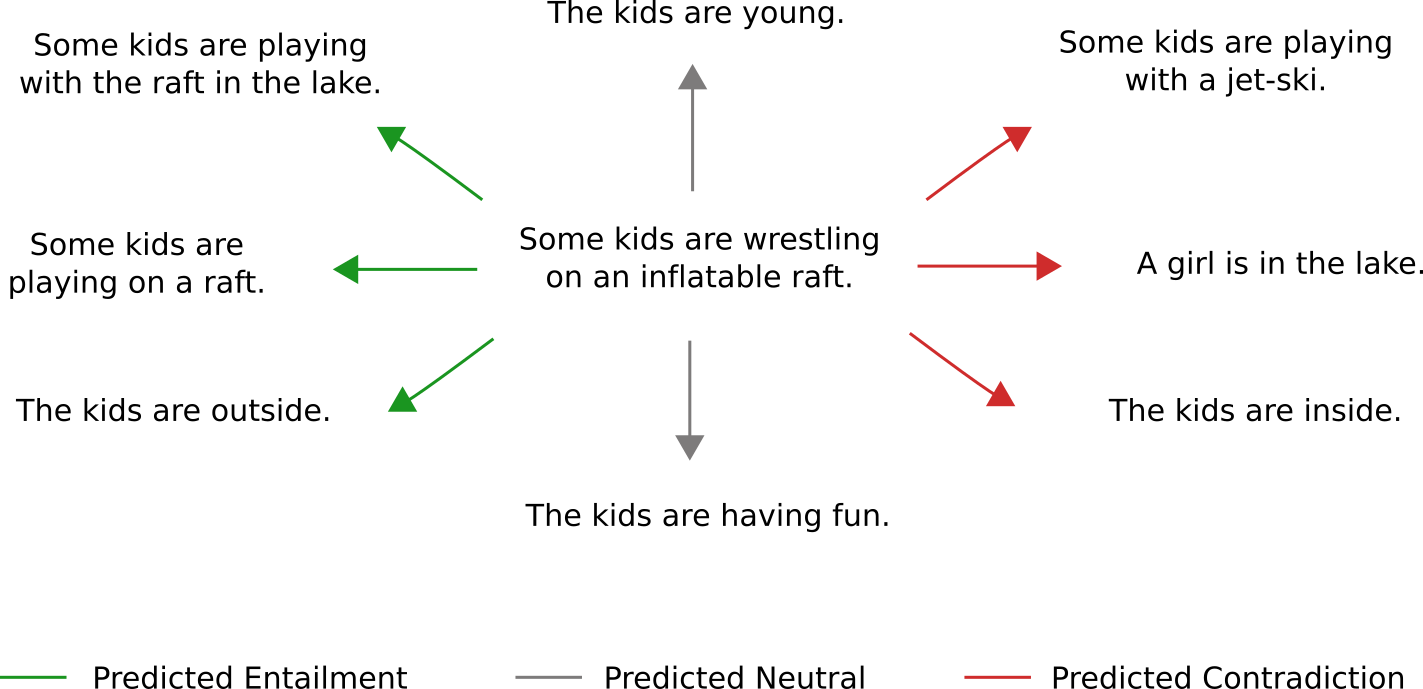
\includegraphics[scale=0.53]{figures/inf-role.png}
	\caption{A modeled estimate of part of the inferential role for the test sentence ``Some kids are wrestling on an inflatable raft.'' The network is constructed by using a tree-structured model trained on SNLI to predict a class label for each sentence pair connected by a colored arrow.}\label{fig:infrole}
\end{figure}

\subsection{Discussion}

On what grounds then is it acceptable to treat the embeddings used in these experiments as having semantic significance? An embedding for a sentence is clearly not something from which one can simply ``read off'' a meaning or a description of the world. Rather, an embedding is something that plays a functional role in a model that exhibits some kind of semantically interpretable behavior. So to answer the question: if a model's behavior can be characterized using intentional vocabulary, then it is appropriate to describe the embeddings that bring about this behavior as meaningful entities rather than mere system states \citep[see][]{Dennett:1987}. 

By this measure, the embeddings produced in the preceding experiments are somewhat semantically degenerate. A model that predicts inferential relationships between sentence pairs is subject to only a very limited form of intentional interpretation. If, for instance, the model produces an entailment prediction, then it is possible to say that the model ``thinks'' that the second sentence it was presented with follows from the first. More generic intentional state attributions are also possible. For example, the model tends to get ``confused'' by quantifiers, and it generally ``assumes'' that sentences with a large degree of lexical overlap entail one another. Such generic attributions also license high-level predictions about how the model will behave in novel situations. It is reasonable, for instance, to expect that the model will make an incorrect prediction if it is presented with lexically similar sentences with subtle quantificational differences (e.g., ``Some apples are rotten'' vs. ``All apples are not rotten''). Overall, though, this sort of intentional interpretation is a bit of stretch.

I am accordingly not arguing that the models just discussed are genuine intentional systems. Rather, I am arguing that these models codify the meanings of the sentences they process only insofar as they can be interpreted as intentional systems. Such interpretations can be more or less successful. But in the ideal limit, if a model can accurately determine what a sentence follows from, what follows from it, and what it rules out, then it counts as genuinely understanding what the sentence means \citep{Brandom:1994}. Meeting this standard of competence is exceedingly difficult, but the models I have just described arguably offer a step in the right direction. And insofar as these models count as comprehending certain sentences, I think it is fair to conclude that the models codify the \textit{meanings} of these sentences. Why? Because the models provide a formal specification of what ought to be expected from the use of particular sentences in terms of various inferential relations. Such a specification, as argued in Chapter 1, is exactly what a theory of meaning aims to provide.

\section{Conclusion}

There is no exact logic of ordinary language, but to admit as much is not to deny the possibility of technically sophisticated analyses of the behavior of linguistic expressions. To give an account of an expression's meaning is to provide a specification of the expected consequences of its use, and the results described in this chapter illustrate how such specifications can be made mathematically precise in terms of embedding models that inferentially relate sentences to one another. More specifically, error-driven function approximators can be used to induce functions that accurately predict inferential relationships between arbitrary pairs of sentences. These functions can also be used to iteratively construct a simple network of inferential relations involving a target sentence, as shown in Figure \ref{fig:infrole}. The goal of the next chapter is to build on this foundation by introducing more sophisticated models that are capable of realizing a broader range of intentionally interpretable behavior. 